\subsection{Class Heterarchy} 
% Author: Clint 
Since, our representation of semi structured query [citation needed] is in OWL ontology format, and our aim is to compare and rank the queries in this format, we had to define a similarity measure between ontologies. The defined ontology class comparison measure "class divergence" [citation needed] assumes that we have an ontology store with unambiguous interpretation of classes and strict hierarchical subclass super class relationships and the classes to be compared should belong to it. We cannot find any robust existing ontology library of that nature for this purpose. So we decided to build a new ontology store and as an initial step the categories from DBPedia store [citation needed] are used. Even though, some of these categories are loosely coupled and not fully agreed upon the sub category and super category relationships, this DBPedia has enormous amount of data in linked form [citation needed]. The OWL ontology [citation needed] format is followed in this process. The DBPedia categories are converted into OWL ontology classes and the super class - sub class relationships are built using the OWL super class sub class axioms [citation needed]. Another reason for selecting OWL for this purpose is that we can make use of the existing APIs for building and reasoning [citation needed] the ontology relationships.


%-------------------------------------------------------------------------------



\subsection{Associating Terms with Categories}
%joir-dan
Once the semantic hierarchy is created, the next step is to create training data for the system. The task is then to grab the pages, build a corpus relating to a given category, and then compile the information in a meaningful way. The overall goal is to grab enough information to properly characterize a category while limiting the amount of unnecessary content within the corpus. The problem with this approach is the page density varies greatly across the heterarchy. Each category within the DBpedia/ Wikipedia heterarchy contains a set of information pages, P, that correspond to concepts that share said category. Considering that the categorical structure is a directed acyclic graph \cite{Suchanek07yago:a}, we consider the use of a Markov Blanket \cite{Friedman97bayesiannetwork} in describing a particular category. The category's that The assumption is that a node can be fully described by its ancestor, descendant, and spousal nodes (parent node of subcategory not equal to the category). While this does not completely solve the issue of a category residing in a sparse area of the graph, the amount of information that can be obtained per blanket is usually more helpful than per category.

% figure: abbreviated Markov blanket for the category Basketball  
\begin{figure}[t]
\centering
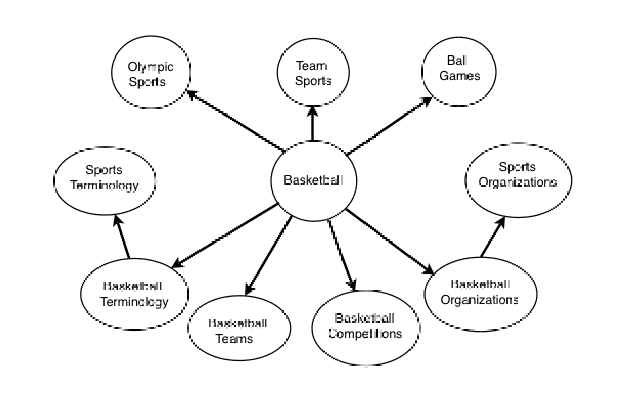
\includegraphics[width=90mm]{abbrv_bb_blanket.eps}
\caption{Abbreviated Markov blanket for the category Basketball}
\label{fig:abbrv_bb_blanket}
\end{figure}

The subcategories of the category Basketball (... Basketball Organizations, Basketball Competitions, Basketball Terminology, Basketball Teams...) can be seen as grabbing information specifc to the category. The supercategories (Ball Games, Olympic Sports, Team Sports) place the category in a higher perspective, abstractly describing basketball as a concept. The spousal categories are an abstract description of the subcategories.

Clustering the categories alone does not guarantee adequate corpus creation. Since the above model relies on the subcategories to describe specifcs of a given category, the ideal situation would be that the subcategories have many more pages than the supercategories and that there is a signifcant amount of information per page. In the case of Wikipedia, there are an average of 25.7 pages per category \cite{1321474}. The assumption for collecting the training data is the more subcategory data we have, the more detailed our description of our category. Considering that there are many categories that have much more than 26 pages, we instituted a PlusOne mechanism to extract extra information. This mechanism checks if a subcategory has an adequate number of pages a to fully describe its subtopic. We set this number to 10 * average, or 39. level represents how many extra levels we are to go down in the hierarchy, if necessary. SubjectSet is the overall set of all pages associated with the blanket structure along with any plusOne subjects obtained.


The overall mechanism does not take into account the amount of information within each page, but generally that can be ignored when considering the size of the blanket corpus when we extract the text from the Wikipedia subject pages. Using this method on the category Basketball, we can construct a corpus of 1843 subject pages and 1,301,006 terms.

When a category's corpus is built, we then build our n-gram frequency distributions and store them in a database for the NLP processing.
